

\section{Motivation}

In times of cloud computing where computer resources are expected to be readily available from anywhere and with an ever growing global network of interconnected devices cloud providers need to cope with increasing energy consumption in data centers as requests need to be handled at a rapid pace \cite{buyya2009cloud}. 
As energy consumption is directly mapped to energy costs, cloud providers aim to reduce power consumption and thus electricity costs within data centers. 

Energy consumption, related energy costs and high energy prices may slow down or hinder advancements in cloud computing. Thus, cloud providers must ensure that delivering their services remains profitable. Lower energy costs increase the competitive ability of cloud providers and bigger investments are possible. Likewise customers may benefit from more affordable cloud services. 

In a study from 2011 \cite{koomey2011growth} global data center electricity consumption amounted to about 1.3\% of the world's total electricity use. This amounts to a total energy usage of 198.8 Terawatt Hours by data centers in 2010. Surprisingly, Google's energy consumption in data centers added up to less than 1\% of that amount. This may be due to Google's constant improvements in energy efficiency \cite{google2015dc}. %\footnote{\url{http://www.google.com/about/datacenters/efficiency/internal/}}. 
When comparing the time period from 2000 to 2005 with the period from 2005 to 2010 data center electricity use increased only moderately due to applied virtualization and other efficiency measures \cite{koomey2011growth, koomey2008worldwide}. Still energy costs of large distributed systems are significant and further actions need to be taken to ultimately reduce these costs \cite{qureshi2009cutting}.

Studies of regional data center energy consumption come to similar conclusions \cite{bitcom2014study}.%\footnote{\url{http://www.bitkom.org/files/documents/Kurzstudie__Borderstep_l_Rechenzentren.pdf}}. 
Through improvements in hardware and cooling systems energy consumption can be further reduced. In addition "`Green IT"' Scenarios can be applied which depend on energy aware routing mechanisms and virtual machine migrations to decrease power usage and costs \cite{liu2009greencloud}. 

Another approach to reduce energy consumption is to reduce cooling costs, since they represent a significant part of the overall energy expenses \cite{patterson2008effect}. This is typically done by installing a more efficient cooling system or by building data centers at locations with low ambient temperature. Cooling through natural powers may also be achieved by building data centers at rivers and using the water to cool down the hardware infrastructure. 

In general energy cost reductions in data centers can be addressed by utilizing one of two different approaches. One common approach is to increase energy efficiency to reduce energy consumption and therefore energy related costs as well \cite{lee2012energy, beloglazov2012energy, berl2010energy, buyya2010energy}. This is done e.g.~by utilizing more energy efficient hardware, implementing an energy efficient cooling system, virtualization of servers or energy aware load distribution policies \cite{patterson2008effect, liu2009greencloud, berl2010energy}. It additionally aims at minimizing the Power Usage Effectiveness (PUE) of data centers which is a term for describing the ratio of the total amount of power consumed by a data center to the power consumed solely by IT equipment \cite{avelar2012pue}. 
Despite the importance of increasing energy efficiency to reduce costs and environmental load this approach is limited as a data center's lifetime cost may not be further reduced when capital expenditures (CAPEX) exceed possible savings in operational expenditures (OPEX) (Figure \ref{fig:decrease_of_pue}). 


\begin{figure}[htbp]
	\centering
		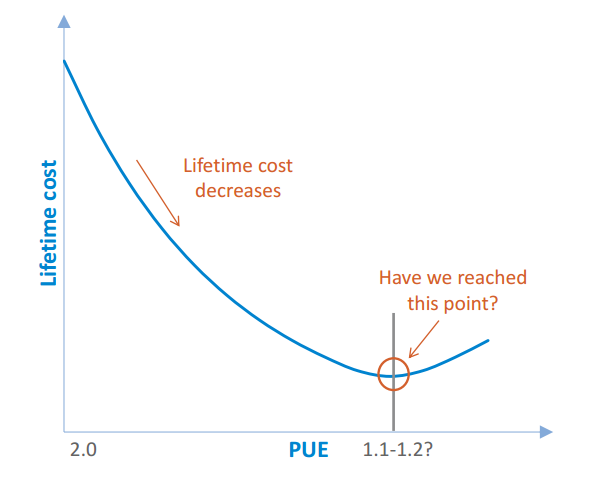
\includegraphics[width=0.70\textwidth]{figures/introduction/decrease_of_pue.PNG}
	\caption{Data center lifetime costs as function of PUE \cite{dcw2013optimizing}}
	\label{fig:decrease_of_pue}
\end{figure}


The second approach is directed at reducing costs by applying intelligent scheduling mechanisms in geographically dispersed and interconnected data centers \cite{guler2013cutting, qureshi2009cutting}. Thus resources are placed at or migrated to locations where the estimated resulting energy costs are lowest. 
An emerging and interesting field of application are cost reductions in data centers connected to wholesale power markets \cite{rao2010minimizing}. These markets provide power prices that change frequently and exhibit high volatility with price differences of factors up to ten between two consecutive observations. 
Electricity price behavior of different power markets may differ substantially as each power market is run by independent operators and exhibits location dependent demand and supply patterns \cite{mugele2005stable}. In addition possibly involved seasonality patterns may lead to substantial locational price differences. For example, considering daily seasonal patterns and data centers located at different time zones these patterns may be exploited to route requests to more cost effective locations. 

These characteristics of locational and temporal varying energy prices may be exploited by intelligent scheduling algorithms and cost aware resource management routines that place requests at facilities currently exhibiting low energy prices \cite{rao2010minimizing}. In addition there is the possibility of migrating resources for sufficiently long running jobs to data centers that operate below peak load and facing low energy prices \cite{buchbinder2011online}.

The focus of this thesis is to go beyond intelligent scheduling of resources by integrating sophisticated forecasting methods that predict price time series behaviors into the near future. This measure is expected to further optimize resource distribution across data centers by comparing and analyzing current and predicted energy price time series to find the best fit of resources in the near future to result in maximum possible energy cost reduction.

%The proposed approach is to optimize load placement and migration between data centers considering time and location based energy prices. 
%In addition to placing resources at locations currently facing low energy prices the resources or virtual machines are migrated to sites where low energy prices are \emph{expected} in the near future. 

%The scenario includes data centers located in different countries where different energy markets and prices apply. Thus constellations may arise where it is profitable to migrate a certain amount of resources from a data center facing high energy prices to a data center where energy prices are low at the current point in time or in the near future. 

\section{Problem Statement}

Reducing operational costs in geo-distributed data centers can be achieved by either increasing energy efficiency of data center components, reducing energy consumption by intelligent scheduling algorithms or finding a way of exploiting cheaper energy prices. In this work a combination of the two latter approaches is applied where regional energy price differences are fed to scheduling algorithms that decide on actions to reduce energy costs. 

Since energy prices change dynamically a flexible approach of moving data center resources to more cost-effective locations is needed. This work is based on the scenario of a company running data centers distributed across several countries. Depending on the current and estimated energy price for a certain region resources may be relocated to other data centers located at more cost-effective regions.

The key technology to implement the relocation of data center resources is virtual machine (VM) migration \cite{nelson2009virtual}. All data and services are located on servers and belong to specific virtual machines within a data center. Since a server may host several VMs that operate completely independent from each other, they can be relocated (migrated) to other servers, possibly over networks without affecting VMs running on the same server. VM migration may be applied across large geographical distances (geo migrations) by leveraging connections across dedicated networks. It is also possible to apply live migrations on a large scale without noticeable service interruption \cite{celesti2010improving}\cite{liu2013performance}\cite{akoush2010predicting}. 

Various load policies exist to optimize the load factor and distribution of tasks within data centers \cite{buyya2010energy,mishra2012dynamic,xiao2013dynamic,pawar2012priority}. A workload manager has to make sure that there are still servers having enough resources and no service level agreement (SLA) is violated on the assignment of a new job. 
In contrast, this work aims to optimize workload distribution among geographically distributed data centers with a focus on the reduction of overall electricity costs. This is done by intelligently scheduling resources while utilizing forecasting methods and predicting energy prices within the near future. 
Furthermore, by considering the history of energy prices and resource load within a certain region it is estimated whether or not a migration to another data center makes sense regarding the current load and configuration. Therefore, forecasting methods in combination with advanced scheduling techniques will be evaluated and applied to the scenario. 

Several challenges arise when aiming to increase cost effectiveness in geo-distributed data centers. First, energy prices are traded and change frequently within energy markets, thus intelligent algorithms have to be provided to benefit from energy price differences across different locations. This is challenging as differences in energy prices can be substantial within a very short time frame which is why the potential benefit of migrating resources across large geographical distances has to be estimated beforehand. 

Second there may be additional cost implications when applying live virtual machine migrations across large geographical distances such as increased bandwidth costs and SLA penalty costs. Depending on the agreed service level agreement the downtime resulting from virtual machine migration must not exceed a defined threshold, otherwise penalty costs are paid to the customer operating the VM depending on the amount of total downtime experienced by the VM. 

Therefore sophisticated methods need to be applied to handle the trade off between exploiting currently cheap energy prices and minimizing migration overhead and costs. This is done by analyzing historical price data and building models for accurate energy price forecasting. Energy prices belonging to different energy markets are estimated for various time ranges into the future. Based upon the results it is decided how many resources may be migrated currently or in the near future in order to obtain the maximum possible energy cost reduction. 

%However, forecasting errors represented by the difference between estimated and real energy prices increase with the length of the estimation window which has to be taken into account when determining the length of the forecasting window. 

%In addition to additional energy and bandwidth costs that arise due to virtual machine migrations penalty costs may have to be paid when the total downtime experienced by a virtual machine exceeds a certain threshold defined by the applicable SLA (service level agreement). 
%so investigations need to be made in order 
%to make qualified statements about the estimated energy price at some point in time in the near future.


\section{Aim of the work}

The goal of this thesis is to reveal possibilities of energy cost reductions for data center operators in charge of geographically distributed and interconnected data centers by exploiting VM migrations and the variability of energy prices in wholesale power markets. This approach presumes that data center operators are charged directly by wholesale power markets, which is becoming a more popular option since it provides a possibility for large cloud providers to ultimately reduce energy costs \cite{dcw2013optimizing}. 
Given the fact that data centers consume a huge amount of energy comparable to the energy consumption of whole cities\cite{qureshi2009cutting} it becomes a viable option for data centers to be integrated into wholesale energy markets. By leveraging the technique of resource migration to data centers where cheaper energy prices apply at the current and future points in time significant savings in energy costs are possible while still maintaining a defined level of quality of service. 

Initially placing resources at data centers that currently exhibit cheap energy prices can reduce energy expenses significantly compared to a non cost aware approach. Combined with energy price forecasts resources may be scheduled intelligently such that price changes within the near future can be detected and resources are placed with respect to the estimated prices. In addition resources may be rescheduled to consider changing energy prices within the current point in time and the near future. 
 
However, different criteria may play a role in determining the most suitable VMs to migrate at the current point in time, or in deciding not to migrate at all. For instance, expected sla penalty costs, bandwidth costs or estimated migration energy can affect the decision of placing or migrating VMs to different data centers. 

These criteria are customizable to provide a means for cloud providers to set preferences for individual criteria over others. For example, a cloud provider may put a high weight on sla penalty estimations to prevent penalties as opposed to emphasizing energy cost reductions which implies a higher probability of sla penalties. 
This approach provides maximum flexibility in focusing on criteria that matter most regarding a specific cloud scenario. 

In addition to the aforementioned goals a focus of this thesis is to provide good quality forecasting for energy price data. Since energy prices in wholesale power markets may be of very volatile nature it is essential to accurately predict prices in the near future in order to obtain maximum cost savings when migrating resources between data centers. 


%These criteria among others are evaluated and applied to the scheduling algorithm to obtain maximum cost reductions. 

%A special focus will be laid on evaluating energy price forecasting methods to find the best fit for the given data and scenarios. For the simulation there will be a focus on short term price forecasting, as energy price levels change rapidly within energy markets and exhibit a very volatile nature. Therefore energy price forecasting is most accurate when applied to short term forecasts. 
%
%Different forecasting methods will be compared by accuracy and error measures to determine the most suitable forecasting horizon and parameter settings for various models and data. It is expected that through good quality forecasting the results of the simulation in terms of energy costs can be improved significantly. This should help cloud providers to save on their energy bills and provide more efficient scheduling of cloud related data. 

\section{Methodological Approach}

As preparation for the simulation and forecasting scenarios different types of electricity price data from various locations is analyzed and relevant characteristics are discussed. Also different energy markets are introduced where each market has its own unique characteristics that can be used for building forecasting models. Also a case study about energy price time series used in this thesis is presented to see differences in real world energy price data of different types and in different locations. 

An evaluation of forecasting methods is performed in order to make qualified assumptions about suitable models for real time and day ahead energy price data. An algorithm for automatic model selection has been implemented that determines possible frequency (seasonality) in the data and generates ARIMA models with suitable parameters based on the data. The resulting models are then evaluated based on a weighted function of corrected Akaike information criterion (AICc) and Ljung box values to determine the most suitable model for the given data. 

To determine the best type of model for a wider range of electricity price data a comprehensive simulation of forecasting models over an extended time range is performed that reveals behavior of models for different types of electricity price data. Models are trained based on different training data sets and exposed to various forecast horizons where the resulting models are compared by a range of error measures (e.g.~MAPE, RMSE). Thus the best model can be determined by comparing resulting error measures whereby the model with the least overall forecast error and most stable distribution is taken as basis for further simulations. 

A simulation scenario will be established where different types of workload is placed on several geographically distributed and interconnected data centers and results are evaluated based on the given workload, energy prices and data center capacities. In addition, energy price forecasts will be integrated to predict significant changes in energy price levels at different energy markets. This leads to a more cost efficient scheduling approach where workload is placed at data centers that provide best energy price conditions for current and/or future time spots. 

The simulation will be based on a well established cloud simulator \cite{lucanin2015philharmonic} with a set of parameters to simulate predefined scenarios. 
The results for different scenarios and parameter settings (e.g.~with or without forecasts) will be compared and evaluated such that the possible benefits of each scenario are revealed. 

The core of the simulation consists of the energy price scheduler which implements different scenarios and a utility function for simultaneously evaluating different criteria to determine the VMs that are most suitable to be migrated at the current point in time. The weights of each utility value may be adjusted such that different scenarios with emphasis on different criteria may be simulated. 

%This evaluation is applied to real price data from various energy markets over a specified time range and results are compared based on different forecast accuracy measures (e.g.~MAPE, RMSE). The best model obtained from this evaluation will be used as basis for energy price forecasting within the simulation. 


 %the used data is analyzed to provide an overview of energy price time series characteristics of different energy markets. 


%The proposed scenario consists of an established cloud with data centers located in countries where participation in power markets is possible and energy price data is available. The geographical location and connections between data centers is defined such that VM migrations may be done interchangeably. 
%
%To maximize the predictive accuracy of price forecasting different parameters of forecasting methods should be evaluated and compared to determine the settings with the most accurate results in each case. The accuracy should be evaluated for models based on different trainings data sets on both in-sample and out-of-sample forecasts and each location and time series separately. Due to the volatile nature of hourly real time energy prices there is a natural boundary of about 48 hours up to which forecasts can be made with reasonable accuracy. Models should be trained and compared based on a weighted function of corrected Akaike information criterion (AICc) and Ljung box p-vlues to determine the most suitable model for the given data. 
%%forecast error measures on in-sample data (i.e.~MAPE)
%
%As a next step a model is to be defined for the simulation with parameters needed for further operation. For example, the amount of bandwidth between two data centers needs to be set and a model for calculating the energy and cost of VM migration has to be defined, depending on current energy prices. Furthermore a threshold for the minimum number of VMs should be set that may be migrated in order to compensate for migration costs. 
%
%Regarding forecasting models there is evidence that some models are generally more suitable for energy price forecasting than others \cite{weron2008forecasting}\cite{weron2005forecasting}. For example, for averaged short term forecasts a common model to use is simple exponential smoothing (SES) which averages out any variations in the data and provides a good stationary estimate of future data values. In many cases this generates results with sufficient accuracy due to a strong irregular component (random fluctuations) in the data set. 
%
%Another common model for price forecasting is the ARIMA model which may contain both an auto-regressive (AR) and moving-average (MA) part and can thus be applied to various data sets depending on the chosen parameters. An advantage of ARIMA models is the possibility to also include trend and seasonal forecasting components. 
%Therefore representatives from each of these models will be chosen with a focus on hourly day ahead and real-time energy prices and comparison of results to estimate the most suitable models for a given dataset. 

\section{Structure of the work}

The structure of this thesis consists of the following sections: 

In the \textit{introduction} a general outline is described comprising the purpose of the thesis, the problem statement and how these problems are solved within the thesis. Short insights are given into proposed methodologies and how they are expected to provide improvements to the outlined scenario. 

\textit{State of the art} discusses relevant literature in the field with a comprehensive collection of related articles and journals. It is examined what kind of advancement in the different fields have been made in the past that relate to this thesis and how they can be used as a basis for further investigations. 
%After a detailed analysis of the different approaches of solving problems in the respective field the approaches are compared and summarized to discuss what is still missing and can be improved upon or further investigated. 

The chapter about \textit{data analysis} provides insights about real world electricity price data, characteristics and differences of energy markets and an electricity price case study is presented to evaluate the type of data that is dealt with in this thesis. 

In the \textit{forecasting} chapter different forecasting models are discussed where the basic model building process is described and an autamated model selection algorithm is introduced. Furthermore different models are evaluated across a wider range of electricity price data and compared by forecast accuracy measures. 

Then the \textit{simulation framework} is introduced where details about the architecture and implementation of the simulation framework are revealed. 

In \textit{Evaluation and results} various simulation scenarios are introduced and results are shown for each type of scenario. 

Finally the thesis concludes with a discussion and future work. 

%Methodology comprises definitions and concepts used in further chapters and provides the basis for the discussion of the proposed solution. It investigates in detail theoretical models and concepts which were derived from extensive research in the field. It gives an overview of different energy markets, their inherent characteristics and related energy price time series behavior. The characteristics of electricity prices in wholesale power markets is discussed, as well as different pricing models applicable to these markets. State of the art data centers are investigated to get an idea of the possibilities and limitations of these systems. Finally relevant forecasting models and their theoretical background are discussed to better understand their applications within the thesis. 
%
%The suggested solution or implementation shows the results and outcome of the research in previous chapters. It comprises the general idea and background for the proposed approach, a description of the technical architecture and structure of the implementation and possible interaction with other systems or components. The model selection process is explained in detail and how it contributes to the overall solution. This is crucial as good quality forecasting depends on the goodness of fit of the model in relation to the given data or time series. The empirical evaluation chapter describes the application of selected models to the framework and its behavior when assigned to real world data from different power markets. 
%An important part of the evaluation is done on a simulator that mimics a cloud environment consisting of several distributed data centers. Considering changing energy prices, ambient temperatures, cooling efficiencies, scheduling of virtual machines combined with energy price forecasting it can provide comprehensive insights on possible cost reductions by applying forecasting in cloud environments. 
%
%The discussion and critical reflection contains an overall discussion and investigation of the proposed solution and its possible benefits and limitations. It is compared to related work and how it fits into current research topics. Potential improvements to the proposed implementation are discussed with a reference of open issues. 
%Finally the results are summarized and potential future advancements in achieving cost reductions in cloud environments are estimated. A future outlook concludes the work. 


